Our goal in navigating the space of possible designs was first and foremost to ensure that the product would be highly performant. To achieve this, we chose to store translated code indefinitely, which allowed us to make certain optimizations when translating jumps and simplified the design overall. Flags are evaluated lazily over the scope of multiple blocks. We do not emulate memory for the guest and link oxtra itself to a high, usually unused address instead. Blocks similar to super blocks but with multiple entry points are used as base unit of translation to reduce the number of links to other blocks.

To ensure we met the time constraints and for our programming pleasure we chose an object-oriented approach in C++, allowing us to divide our source code into classes for ease of navigation and to work concurrently on the project without fear of intersection.

To decode x86-64 instructions, we have decided to use fadec\footnote{\url{https://github.com/aengelke/fadec} (visited on 12/10/2019)}, a 32 and 64 bit compatible decoder, written in C and adapted by us to be object oriented for easy use in oxtra. For logging, we use a small wrapper for fmt\footnote{\url{https://fmt.dev/latest/index.html} (visited on 12/10/2019)}.

\subsection{Architecture Overview}
	The implementation of the translation process is abstracted by the dispatcher. To start the translation of a binary only a \texttt{Dispatcher} object has to be created, which internally manages all the other components of the architecture. To initiate the execution, \texttt{run} is called on the dispatcher object. \texttt{run} returns the return value of the translated program, once the execution is finished.

	\subsubsection{Internal Block Structure}
	To translate code sections, oxtra splits instructions into chunks which are advanced deviations from super blocks. Those \emph{blocks} are defined as a list of consecutive operations up to the next block ending instructions. Block ending instructions are: \texttt{jmp}, \texttt{call}, \texttt{ret} and \texttt{syscall}. This structure similar to super blocks means, that a block may contain multiple exit points (e.g. conditional jumps). Due to the internal structure and capabilities of the implementation, a block can also have multiple entry points upon creation. This renders these blocks incapable of being called basic blocks or super blocks, as they have a single point of entry per construction.

	\subsubsection{Environment Initialization}
		% in english, long dashses do not have a space
		The initialization process of oxtra is rather straightforward and is illustrated in \autoref{fig:lifecycle-initialization}. Initially, the arguments are parsed and processed with the use of \emph{argp}---not only the arguments that control oxtra itself but also those that will be passed to the guest application.
		
		Afterwards, the ELF file itself will be processed---thoroughly explained in \ref{documentation_elf}---which breaks down into three major steps: opening the elf file, ensuring correctness of essential values, and unpacking the elf file into memory for easy processing.
		
		In the next step, the guest is initialized by setting the context (see \ref{context}) according to the x86-64 System V ABI\footnote{The Application Binary Interface defines low level requirements and behavior specific to a kernel and an architecture.}, mainly allocating a stack for the guest and pushing key values (e.g. argument count, arguments, environment variables \dots) onto it \cite{systemv}. With the guest prepared, oxtra can switch to the new context and start translating the initial code block.
		
		\begin{figure}[htb]
			\centering
			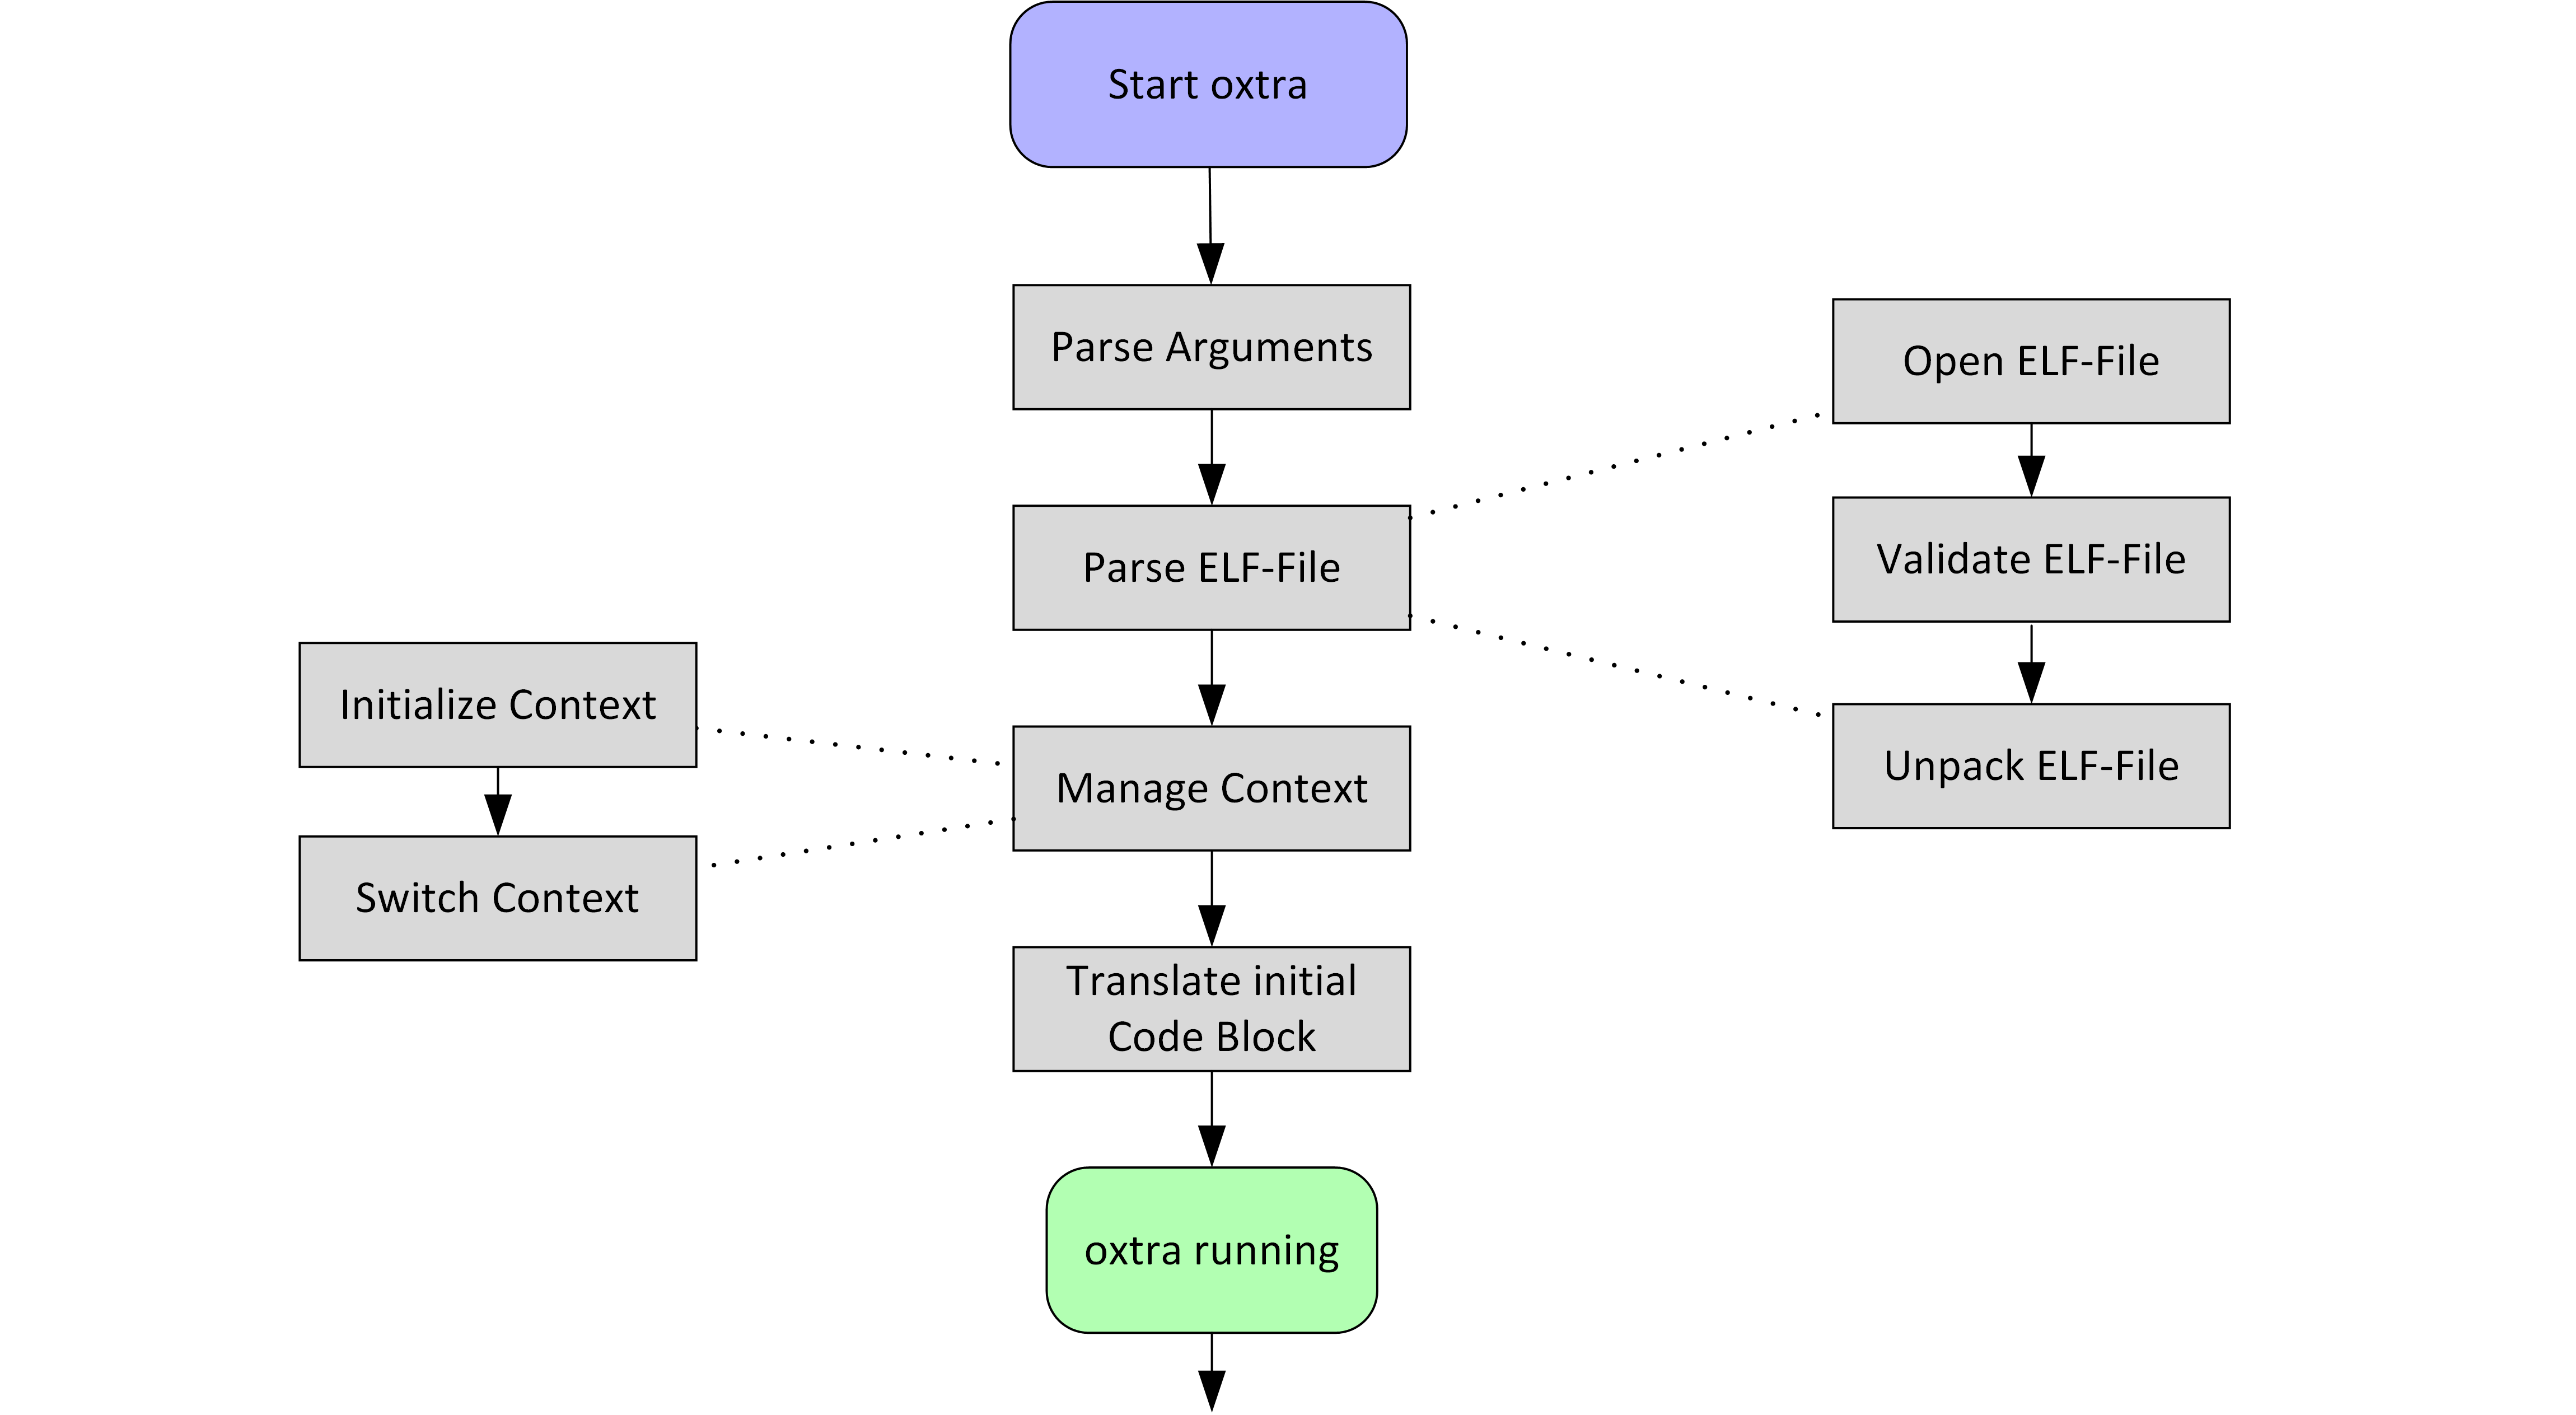
\includegraphics[width=1.0\linewidth]{architecture/lifecycle-initialization}
			\caption[Runtime Initialization]{Initialization of the runtime environment and preparing oxtra for execution.}
			\label{fig:lifecycle-initialization}
		\end{figure}
	
	\subsubsection{Core Processing Cycle}
		After oxtra has been successfully initialized and the first block translated, the translation loop has started. This life cycle, illustrated in \autoref{fig:lifecycle-processing}, begins by executing an initial block, possibly followed by multiple statically linked blocks (see \ref{Block Chaining}).
		
		Eventually, a target of a block cannot be statically evaluated (e.g. an untranslated block or the target is stored in a register), forcing the guest to give control back to the host. After the context of the guest has been stored, the host can fully take over (marked by the dash-dotted rectangle).
		
		The Code Manager ensures that the target address has already been translated. If this is not the case, the block beginning with this address will be translated and stored. After this procedure, the address of the actual RISC-V instruction can be passed to the guest and used as the starting point for further execution. In our implementation, any arbitrary instruction in an already translated block can be referenced and used as a starting point, without the need to duplicate code. 
		
		If the final link in a chain of blocks is a static link, the last block and the new block will be chained \emph{statically} by replacing the switch to the host with a jump directly to the next block (see \ref{Block Chaining}). If it is a dynamic link, the address has to be reevaluated every time the link is taken (see \ref{translating conditional jumps}).
		
		Eventually, an exit system call (or an error) is encountered, marking the end of the execution process and causing the guest to stop. If the error was detected (not all segmentation faults are detected), the context of the host will be fully restored. Finally, the exit code of the guest is returned by the host itself causing the guest and the host to be stopped. 
		
		\begin{figure}[htb]
			\centering
			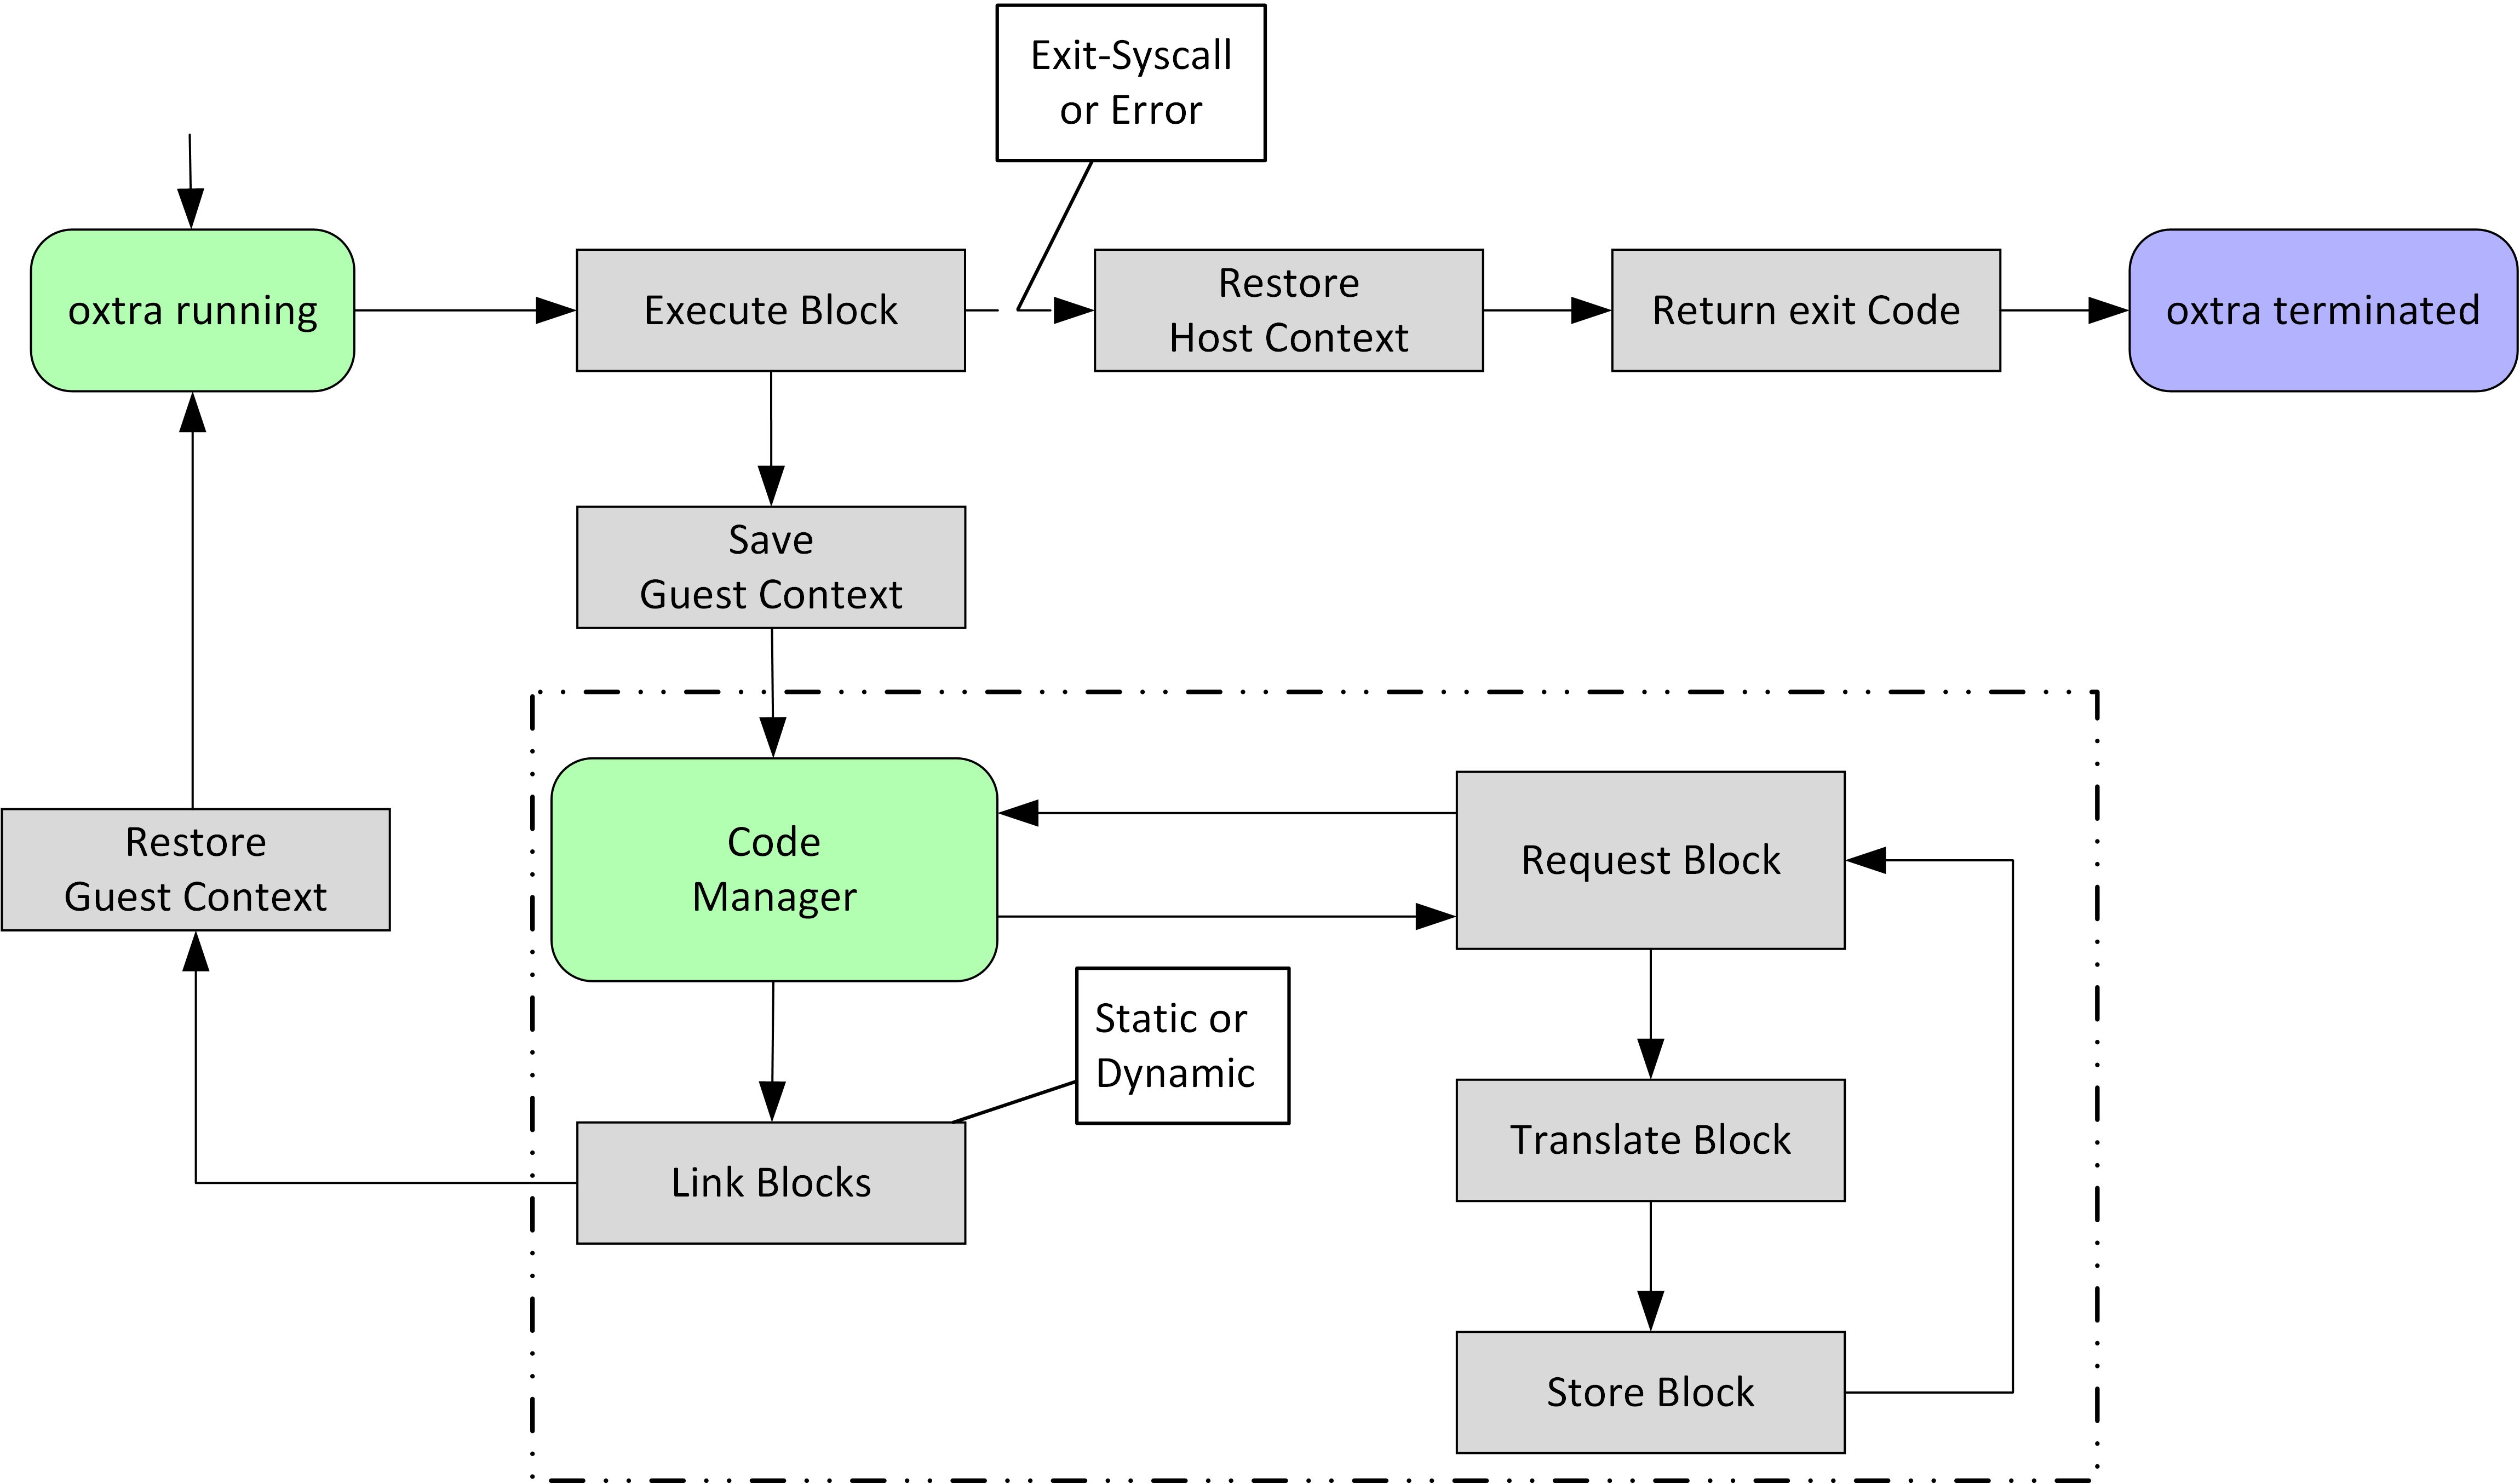
\includegraphics[width=1.0\linewidth]{architecture/lifecycle-run}
			\caption[Instruction Processing]{Processing cycle responsible for translating, executing, and storing instructions.}
			\label{fig:lifecycle-processing}
		\end{figure}
	
	\subsubsection{Component Overview}
		For translating and executing blocks, oxtra requires three core components that have been illustrated in \autoref{fig:component-overview}.
		
		\paragraph{The Dispatcher} implements the interface between the guest and host. Whenever the guest gives control back to the host, a method of the dispatcher is being called. Those methods control the main execution flow like the translation of blocks or the mapping and emulation of system calls. This means that the Dispatcher essentially controls the host.
		
		\paragraph{The Code Generator} translates blocks and generates RISC-V instructions accordingly. Additionally, it controls the flag evaluation process, mainly consisting of selecting instructions that should set flags (lazy evaluation) and ensuring that flags are consistent over multiple blocks.
		
		\paragraph{The Code Store} saves and manages previously translated blocks with a simple paging mechanism. Before generating a block, the Code Generator queries the Code Store whether this block has already been translated. With the current implementation, this caching mechanism does not allow reallocation or deletion of blocks (see \ref{code storage}).
		 
		\begin{figure}[htb]
			\centering
			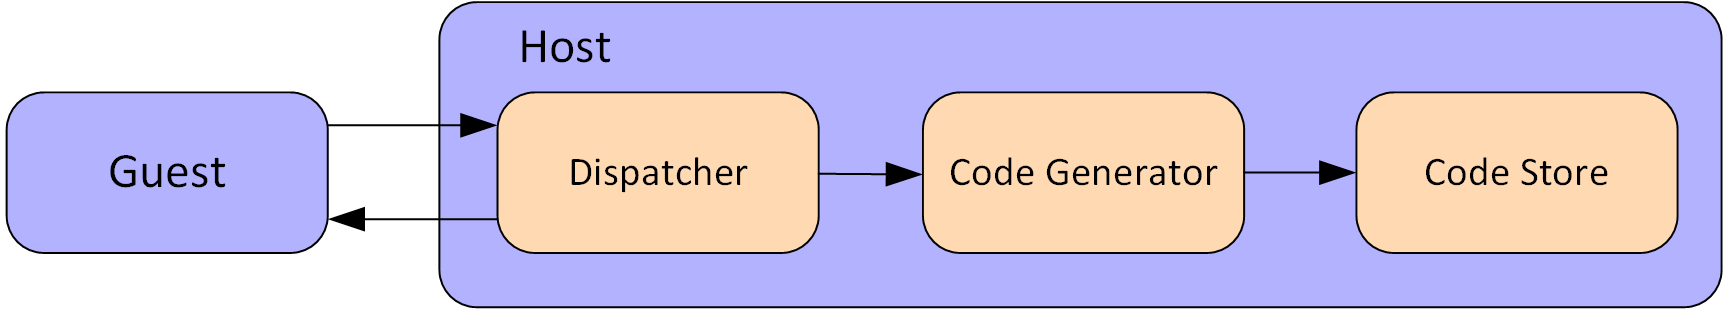
\includegraphics[width=0.75\linewidth]{architecture/component-overview}
			\caption[Component Overview]{Core components participating in the translation and execution process.}
			\label{fig:component-overview}
		\end{figure}

\subsection{In-Depth Architecture}
	The architecture described in the previous sections simplifies many aspects and is meant to be a starting point. It either ignores the underlying system that composes a higher-level component or leaves out some (rather) important parts. The UML class diagram illustrated in \autoref{fig:uml-architecture} fills this gap and shows the actual dependencies and associations between the components/systems, while only leaving out smaller details.
	
	\subsubsection{Dispatcher}
		The two purposes of the main method are to create the dispatcher with all required references (namely elf and arguments) and invoke the translation and execution process by calling \texttt{run}. Once this procedure has been initiated, the dispatcher prepares the \texttt{ExecutionContext} which stores important values for the host/guest (e.g. the contexts), and the execution process (e.g. flag information). Afterwards the first block can be translated, the context switched, and the execution process started.
		
		The dispatcher is not only responsible for setting up the guest, but also functions as the central access point for the guest: whenever supervision by the host is required, a specific method of the dispatcher will be called that decides the further flow of execution. This means that the dispatcher has special entry points for handling system calls and linking blocks that will be called from the generated RISC-V assembly. 
	
	\subsubsection{Code Generator}
		The code generation system (\texttt{CodeGenerator} and its dependencies) provides two main interfaces: translating a given guest address until the end of a block is encountered and chaining previously translated blocks. In theory, this code translation process seems quite straightforward, but many functioning parts are required for the process to work properly.
		
		One essential part is the \texttt{CodeBatch}, which provides a unified way for the instruction classes to store generated instructions. It also allows adding placeholders (e.g. \texttt{nop}s), that are replaced later (e.g. for conditional jumps). Further, the usage of \texttt{CodeBatch} as a generic construct allows us to exchange it with a \texttt{DebuggerBatch} that adds additional instructions and notifies the Debugger of new operations. 

		To translate x86-64 to RISC-V, every x86-64 instruction is implemented in its own class that inherits from \texttt{Instruction}, or, should it make implementation easier, from \texttt{UnaryOperation} or \texttt{BinaryOperation}\footnote{Some similar instructions share a common class (e.g. mul, and imul).}.
		
		In the core translation cycle, the \texttt{decode\_instruction} method of the \texttt{CodeGenerator} is repeatedly called. To decide which x86-64 fadec instruction corresponds to which actual implementation, the \texttt{InstructionTransform} is used. This class provides a mapping method that transforms x86-64 instruction into our implementation. The specific instance then adds RISC-V instructions to the \texttt{CodeBatch}, which are then stored in the \texttt{CodeStore} by the \texttt{CodeGenerator}.

	\subsubsection{Code Store}
		Three essential pieces of information need to be stored for the \texttt{CodeStore} to manage the executable code properly: the actual RISC-V code that can be executed, the address of the x86-64 instructions, and the number of RISC-V instructions per x86-64 operation. With this information, the code can not only be stored but also searched for with \texttt{find(addr)}. By storing the length of every x86-64 instruction, this interface also allows for finding addresses \emph{in} already translated blocks (instead of only finding the address of the start of a block).
		
		It is worth noting that for a block to be executed linearly and as a whole, the code has to be stored \emph{sequentially}. For this we implemented \texttt{StaticList} that can guarantee sequential storage for a given set of data. Additionally, this list also ensures that already translated addresses are not reallocated, preventing blocks from becoming invalid over time.

	\begin{figure}
		\centering
		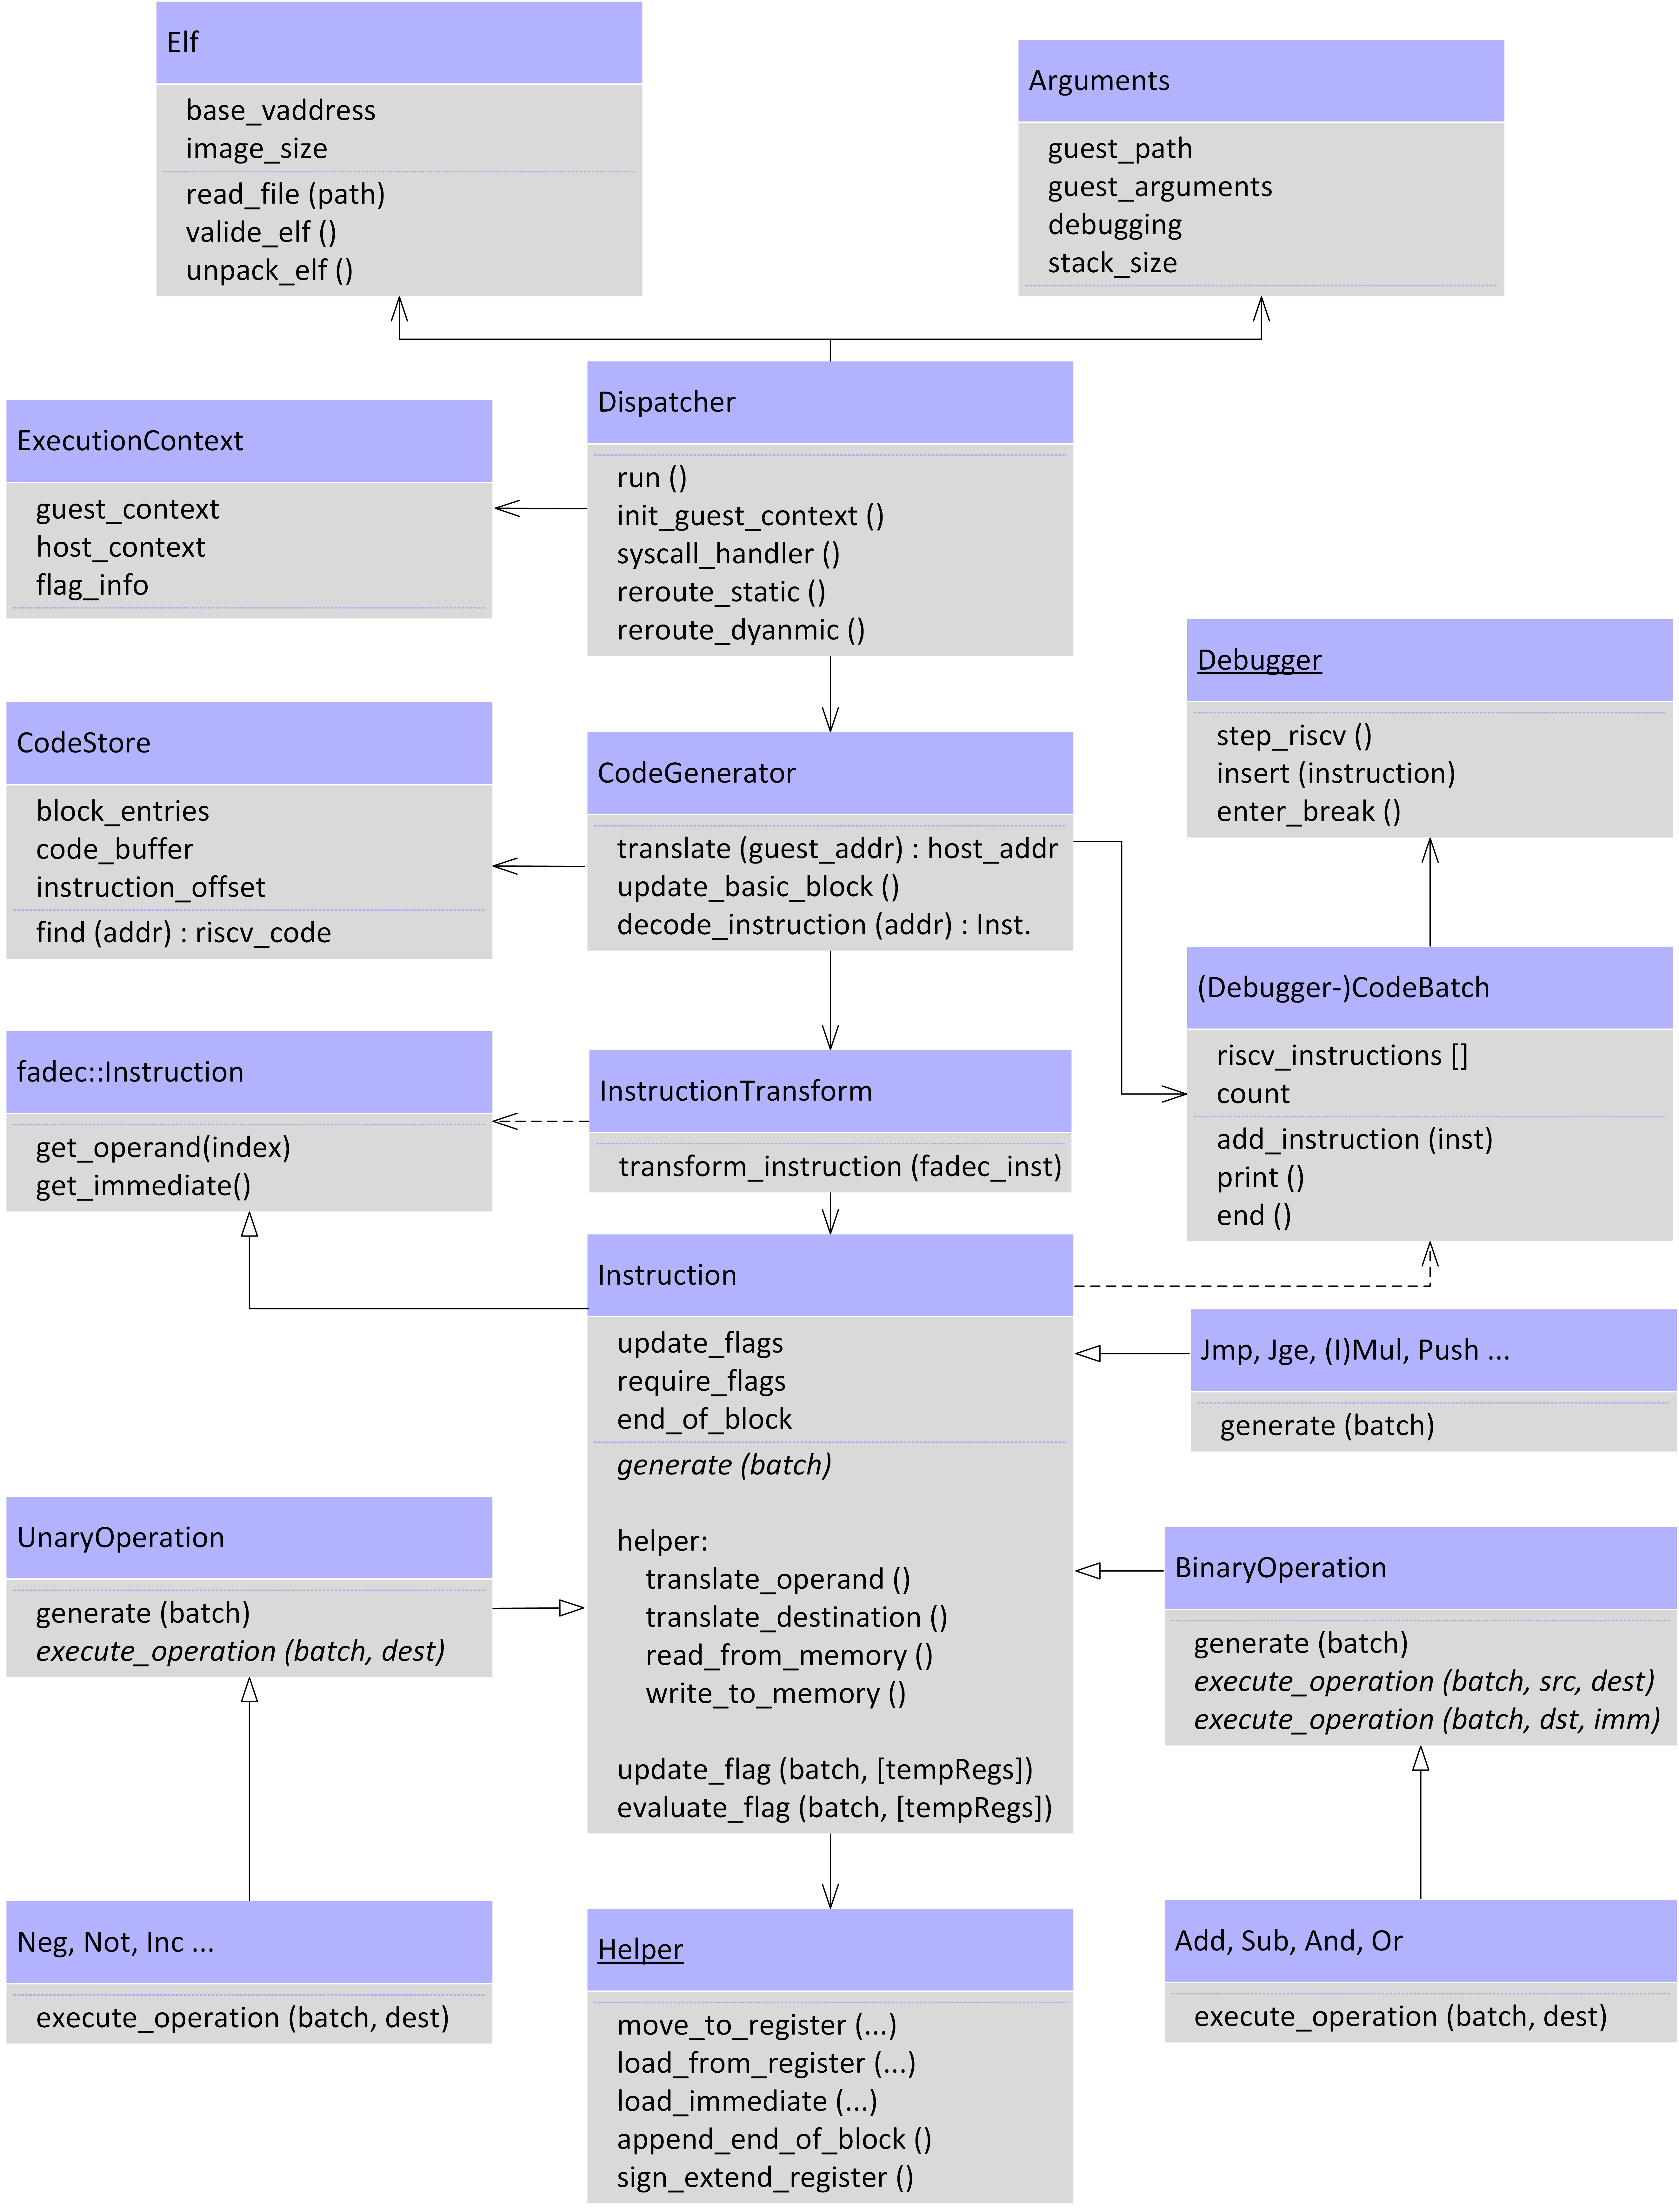
\includegraphics[width=1.04\linewidth]{architecture/uml-architecture}
		\caption[In-Depth UML Architecture]{Architecture of oxtra represented as an UML class diagram.}
		\label{fig:uml-architecture}
	\end{figure}

\subsection{Register Mapping}
As previously mentioned, oxtra maps every x86 register to a RISC-V register. The mapping used in oxtra is illustrated in \autoref{fig:register-mapping}. This mapping has not been chosen arbitrarily, but ensures that the registers for system calls do not have to be moved or altered. The registers \texttt{s1}, \texttt{s8}, \texttt{s9}, \texttt{s10}, and \texttt{s11} store addresses required for execution and will be explained in the following sections. 
\begin{figure}[H]
	\centering
	\begin{subfigure}[b]{.5\textwidth}
		\centering
		\begin{tabular}{|c|c|} 
			\hline
			\textbf{RISC-V Register} & \textbf{Purpose}\\
			\hline
			a7 & rax \\
			a6 & rcx\\
			a2 & rdx \\
			s2 & rbx \\
			sp & rsp \\
			s0/fp & rbp \\
			a1 & rsi \\
			a0 & rdi \\
			a4 & r8 \\
			\hline
		\end{tabular}
	\end{subfigure}%
	\begin{subfigure}[b]{.5\textwidth}
		\centering
		\begin{tabular}{|c|c|} 
			\hline
			\textbf{RISC-V Register} & \textbf{Purpose}\\
			\hline
			a5 & r9 \\
			a3 & r10 \\
			s3-s7 & r11-r15 \\
			s1 & Return Stack \\
			s8 & Call Table \\
			s9 & TLB \\
			s10 & Jump Table \\
			s11 & Context \\
			t0-t6 & Temporary \\
			\hline
		\end{tabular}
	\end{subfigure}
	\caption[Register Mapping]{Specification on the usage of the 31 available registers in RISC-V.}
	\label{fig:register-mapping}
\end{figure}

\subsection{Translating Instructions}
	The primary translation routine consists of four steps: Initial validation, instruction mapping, flag prediction, and code generation.
	
	\paragraph{Initial Validation} ensures that the upcoming address is valid and has not been translated yet. First, the upcoming address is validated against the ELF file to ensure that the new target address is valid and inside the text section. If the address is valid and has not been translated before, oxtra will extract the address of the next upcoming block, which has already been translated, from the \texttt{CodeStore}. Using this upcoming address, the main three processing components are executed.
	
	\paragraph{Instruction Mapping} is the process of decoding the instructions and mapping them to actual instruction classes capable of generating RISC-V code. This process is repeated for every instruction until either a block ending instruction (e.g. \texttt{ret}, \texttt{call} \dots) is found, or an already translated block is encountered. Stopping at a previously translated block ensures that every instruction is translated only once (see \ref{code storage}). 
	
	\paragraph{Flag Prediction} determines which flags each instruction must update. In order to achieve this, two additional pieces of information are stored for each instruction: the flags that the instruction requires for execution (e.g. \texttt{adc} needs the carry flag) and the flags that the instruction alters (e.g. \texttt{inc} updates all flags except the carry flag). To predict which instruction must update a certain flag, the instructions are iterated in reverse order. By iterating in reverse, the instructions which read the flags are encountered before the instruction which would have to update the flag. These are then marked as having to update the given flag. Thus, only the necessary instructions will update any given flag. Additionally, to ensure that flags are consistent over blocks, the instruction that ends the block determines which flags are further required. If the target block is statically linked, the flags will be analyzed recursively (up to a maximum depth) with the next block, reducing the number of evaluated flags. With dynamic links, all flags have to be updated as the next block and it's required flags cannot be predicted.
	
	\paragraph{Code Generation} produces the executable RISC-V code and can be started once the required flags for every instruction are known. Oxtra then begins to translate all instructions inside the current block by calling the \texttt{generate} function of each \texttt{Instruction}. In conjunction with the code store, these translated instructions are written sequentially into memory. \\
	
	\noindent Once all instructions have been translated and stored permanently, the starting address of the newly translated block is returned, and execution can continue.

\subsection{Jump Table}
	\label{Jump Table}
	Jumping to an arbitrary address on RISC-V involves loading the address into a register and then jumping to that address with \texttt{jalr} (possibly up to eight instructions). There are a few addresses that are constantly jumped to during translation and execution such as the methods for statically or dynamically linking blocks, the system call handler or carry and overflow evaluation functions (see \ref{documentation_flags}). These are stored in the jump table.

	The jump table consists of \texttt{jal} instructions which add a signed 20 bit offset to the address of the next instruction and then jump to it, effectively allowing for jumps into a 1 MiB large region around the program counter. The address of the jump table is stored in a register (see \ref{register_mapping}) and jumped to with just one \texttt{jalr} instruction, which encodes a signed 12 bit offset. This jumps to an entry in the jump table which in turn jumps to the corresponding function. The return address points to the instruction after the \texttt{jalr}.

\subsection{Evaluating Flags}
	\label{documentation_flags}
	Oxtra implements lazy flag evaluation, which means that flags are not calculated for every instruction but rather only when they are needed (e.g. in conditional jumps) (see \ref{approach_flags}). This mechanism is implemented by the \texttt{Instruction::update\_flag} and \texttt{Instruction::evaluate\_flag} methods. Oxtra only supports the \texttt{carry}, \texttt{overflow}, \texttt{sign}, \texttt{parity}, and \texttt{zero flag}. The other flags are ignored, as they are either meant for system programming or practically deprecated. The only other flag, which might be interesting is the \texttt{direction flag}. By not implementing the two instructions that can update the \texttt{direction flag} (\texttt{std}, \texttt{popf}), it is ensured that the flag cannot be set, which would lead to undefined behavior.
	An instruction that modifies a flag calls the \texttt{update} method and an instruction that reads a flag calls the \texttt{evaluate} method for that flag. The \texttt{update} methods store values in the \texttt{ExecutionContext} and the \texttt{evaluate} methods read the values from there and calculate the state of the flag. For the zero, sign, and parity flag the \texttt{update} methods store the result of the operation that updated the flag (e.g. the x86-64 \texttt{add} instruction stores the sum of the two input values). The carry and overflow flag calculation depends on the type of operation that updated the flag, so the \texttt{update} methods store an offset into the jump table where the corresponding evaluation function is located, in addition to two input values. The carry and overflow \texttt{evaluate} functions now load this offset and jump into the jump table to the concrete evaluation function.

\subsection{Intermediate Representation}
	Oxtra has been designed in a way that allows fast and easy implementation of new instructions. Because x86-64 has hundreds of instructions, oxtra is not nearly capable of translating all of them. Most of the core instructions of x86-64, (i.e. integer arithmetic, moves, logic, conditional jumps, stack operations) have been translated. But it is still very likely to encounter an instruction that oxtra does not support.
	
	New instructions require three things to be implemented. The instruction has to have its own class which either inherits directly from \texttt{Instruction} or from one of the helper classes (i.e. \texttt{BinaryOperation}). The constructor of the super class will expect flag information (which determines the instruction updates, and which flags the instruction reads), which is relevant for flag prediction, as well as the information whether the instruction will end the current block. Afterwards the instruction has to be added to the switch statement in \texttt{transform\_instruction}, as this will allow the translation loop to instantiate the new instruction whenever it encounters an instruction which is implemented by the new class. The last thing required is to implement the generating code. For this oxtra has a variety of helper functions (mainly in \texttt{Instruction} and \texttt{helper}), which ease the process of generating code. 
	
	\subsubsection{Control Flow Instructions}
		Instructions that can alter the control flow have to implement \texttt{branch\_address} and \texttt{control\_flow\_dimension}. These functions are used by the recursive flag prediction to handle different control flows properly. The function \texttt{branch\_address} should return the address of the alternative control path or 0 if the control path is indirect (e.g. a jump to a register). The function \texttt{control\_flow\_dimension} must return 1 if the instruction just has one control flow, by following a new address (e.g. \texttt{jmp}, \texttt{call}\dots). A return value of 2 indicates that there are 2 possible control flow branches, which is the case for conditional jumps.

	\subsubsection{Operation Types}
		\label{Binary Operation and Unary Operation}
		A lot of x86-64 instructions have the same structure:

		\paragraph{Binary Instructions} contain two operands of which the first operand is both source and destination and the second operand is just a source operand. Either the first or the second operand can be a memory access and the second operand can be an immediate.
		
		\paragraph{Unary Instructions} contain only a single operand which is a both source and destination, which can either be a memory access or a register.\\
		
		Because of this common structure, oxtra implements the classes \texttt{BinaryOperation} and \texttt{UnaryOperation}. Instructions can inherit from these classes, which forces them to implement a function called \texttt{execute\_operation}. The classes \texttt{BinaryOperation} and \texttt{UnaryOperation} take care of loading the two operands into registers as well as storing them back to their designated destination. The two classes are highly optimized, which is the reason why \texttt{execute\_operation} is not allowed to change the contents of the source register. This is also the reason for the registers only having the bits of the operand size right. The upper bits might be cleared or contain other values.
	
	\subsubsection{Register Access}
	Register interaction poses a problem for DBT since x86-64 allows access to parts of registers like \texttt{ah} and \texttt{al}, while RISC-V instructions will always interact with the whole 64 bits. Even though there are instructions that operate on just the lower 32 bits (e.g. \texttt{ADDIW}), they sign-extend their result into the upper 32 bits. For this reason, the two helper functions \texttt{helper::move\_to\_register} and \texttt{helper::load\_from\_register} were implemented, which in tandem provide x86-64 partial register access.
	
	\texttt{load\_from\_register} reads parts of a register and stores it in the lower bits of another register. \texttt{move\_to\_register} can write the lowest bits to a destination register without invalidating the other bits\footnote{32-bit operations on x86-64 clear the upper 32-bits in the destination register.}.
	
	For example, translating \texttt{mov ah, al} could be implemented by calling the helper functions:
	\begin{lstlisting}
load_from_register(src = RAX, access = LBYTE, temp = t0);
move_to_register(dest = RAX, src = t0, access = HBYTE);
	\end{lstlisting}
	
	\subsubsection{Loading Immediates}
	Writing an immediate value to a register is tricky in RISC-V since you cannot encode a 64 bit immediate in a single 32 bit instruction. The most bits you can encode in a single instruction is 20 (\texttt{lui}), but since this instruction invalidates all the bits it does not set you can only use it once per immediate loaded. The other (up to) 44 bits will have to be encoded with a combination of immediate arithmetic operations and shifts, encoding (up to) 12 bits per arithmetic operation.
	
	The naive solution would be to use \texttt{addi} as the arithmetic instruction. However, since \texttt{addi} sign extends, the halfway loaded immediate could be invalidated by each subsequent \texttt{addi}, necessitating corrective shifts. Our function \texttt{helper::load\_immediate} uses \texttt{xori} instead, which will invert the partly loaded immediate instead of adding to it, meaning that instead of multiple corrective shifts we need merely a single corrective \texttt{xori}.
	
\subsection{Call and Return}
	Oxtra optimizes \texttt{call} and \texttt{ret} to avoid calls to \texttt{reroute\_dynamic} which dynamically links blocks. Both reads and writes of the return address value on the guest stack are still allowed by the use of two additional data structures:
	
	\subsubsection{Data Structures}
		The \emph{call table} has an entry for each call in the guest code. An entry stores both the x86-64 return address and the address of the RISC-V code that corresponds to the return address. 
	
		The \emph{return stack} is an additional stack that holds 4-byte offsets into the call table. It is implemented by a ring buffer so that it can neither overflow nor underflow. A \texttt{call} pushes it's offset into the call table onto the stack and a \texttt{ret} pops that offset and retrieves information about the \texttt{call} (e.g. the corresponding RISC-V return address) from the call table.

	\subsubsection{Translation}	
		When translating a \texttt{call}, a new entry in the call table is allocated and the return address is stored. The corresponding RISC-V address is initialized to zero to indicate that this code has not been translated yet. An execution of \texttt{call} will now push the call table offset onto the return stack and the return address onto the guest stack.
		\texttt{ret} pops the return address from the guest stack and the call table offset from the return stack to load the return address from the call table entry.
		Handling \texttt{ret} now involves three cases:
		\begin{enumerate}
			\item If the return address from the call table does not match the return address from the guest stack (i.e. the return address was modified), then \texttt{reroute\_dynamic} is called to transfer control to the modified return address.
			\item If the return addresses match but the RISC-V address is zero, meaning it was not translated yet,  then \texttt{reroute\_return} is called, which translates the code and stores a pointer to it in the call table entry before jumping to the translated code.
			\item If the return addresses match and the RISC-V address is not zero, then a jump to the RISC-V address is performed.
		\end{enumerate}

\subsection{System Calls}
\label{documentation_syscalls}
	When the code generator encounters a \texttt{syscall} instruction it will generate a call to \texttt{Dispatcher::syscall\_handler}, which implements the solution to the two major problems of system calls between different architectures: emulating system calls that either do not exist or have different behavior, and index mapping for system calls that should be forwarded to the host kernel (see \ref{approach_syscalls}).

	These problems are solved using a system call map (\texttt{syscalls::syscall\_map}). A x86-64 system call index is mapped to an entry in the map which either describes a pointer to an emulation function, the index of the system call in the RISC-V kernel, or marks the system call as unsupported.
	
	If the entry describes a RISC-V system call index, then this index is used to issue the system call using the \texttt{ecall} instruction without a need to store the context. The register mapping (see \ref{register_mapping}) was chosen to simplify the translation of the calling conventions\footnote{\url{http://man7.org/linux/man-pages/man2/syscall.2.html} (visited on 15/10/2019) Paragraph: Architecture calling conventions} by mapping the x86-64 register that contains the n-th argument to the RISC-V register that contains the n-th argument.
	
	If the entry describes an emulation function, or marks the system call as invalid, the context is stored and the C++ function \texttt{Dispatcher::emulate\_syscall} is called which either calls the corresponding emulation function or stops the execution due to an unsupported system call.
	
	\paragraph{brk}
		exists on RISC-V but requires special handling. It sets the program break (the end of the data section) and is used by most libc implementations to allocate memory for the heap. If just forwarded to the kernel it would modify the program break of the host, thus it has to be emulated.
		
	\paragraph{arch\_prctl}
		can read and write the base address of the \texttt{fs} and \texttt{gs} segment registers. These are used in most libc implementations of pthreads. The translator stores the \texttt{fs} and \texttt{gs} base address in the \texttt{ExecutionContext} and loads them into a register when there is a memory access with \texttt{fs}- or \texttt{gs}- segment override.

\subsection{Conditional Jumps}
	Conditional jumps split up the control flow: either the condition is true and this jump is taken, which will either be translated to a static or dynamic link depending on the type of jump, or the condition is false and the jump is not taken, which will just continue the execution on the current path. The conditions are expressed in terms of boolean equations that involve flags \cite[Volume 1 Appendix B.1]{x86-64isa}. Since some flags are more expensive to compute in software than others, conditional flags are evaluated beginning with the least expensive flag. For example, the condition for a \texttt{jg} is \((\text{sign flag} = \text{over flow}) \land \lnot \text{zero flag}\). Evaluating the zero flag is less expensive then evaluating the sign and overflow flag, so it is evaluated first and compared to one. Since the equation can never be true if the zero flag is one and thus sign and overflow would not need to be evaluated in that case.

\subsection{ELF}
	\label{documentation_elf}
	Oxtra is capable of loading and mapping statically linked 64 bit ELF files. It starts by loading the given file and making sure the file is an ELF file. It does so by inspecting the files \texttt{executable header}, which stores information about the type of binary and the required architecture. Afterwards it allocates a memory at the address requested by the binary. If the address is already taken by some other data, loading will fail. After the memory has been allocated, oxtra will copy the necessary sections of the binary into the memory. While copying the memory, oxtra also keeps track of the access rights every page should have. Those privileges are stored in an array which is managed by the \texttt{elf::Elf} object. Even though oxtra allocates the chunks with their given access rights, the executable flag would not be enforced, as the code generator will only read the executable data and translate them, thus possibly translating not executable data. To prevent this, the code generator fetches the flags before translation, which the \texttt{elf::Elf} object keeps track of. If these flags prohibit execution, the code generator will exit with the error \texttt{Virtual segmentation fault}. %There is an elf loader in progress, which would be capable of loading dynamically linked binaries, however it is not completed as of now.

\subsection{Debugger}
\label{Debugger}
	As developing software, especially for large and complicated projects, can lead to some minor bugs or unexpected behavior, oxtra ships with a built-in debugger. By default, the debugger is disabled, but can be enabled via the argument \texttt{debug}. The debugger comes in two forms: \texttt{lightweight} and \texttt{RISC-V-enabled}, the core difference being the possible granularity. The debugging interface could also be used to implement a \emph{GDB}\footnote{\url{https://www.gnu.org/software/gdb} (visited on 15/10/2019)} server. However, this has not been done, as the development of the debugger itself required special features and modification of the architecture. With the currently implemented debugger, supporting GDB should be straightforward as most required methods are already implemented. 
	
	\subsubsection{Overview}
		When debugging is enabled, a menu will show up after translating the first block but before executing the first instruction. Once the debugger command line is available, there are several ways to reopen the menu after resuming the execution. Unfortunately, there is no way to regain control if none of the methods beneath has been used.
		\begin{itemize}
			\item Reaching a Breakpoint
			\item Start of Block
			\item End of Block
			\item Stepping (RISC-V or x86-64)
			\item Run counter elapsed
		\end{itemize}
	
	\paragraph{Breakpoints}
		By using the command \texttt{break} or \texttt{bp}, a breakpoint can be set relative to the current address \texttt{break +/-rel} or with an absolute address \texttt{break abs}. Entering the command \texttt{break} itself will list all registered break points. The breakpoints are limited to virtual x86-64 addresses and there can be at most 255 different breakpoints. Breakpoints can be set for addresses that have not been translated yet. Those breakpoints will be free floating until the block has been translated, at which point the breakpoint might be adjusted to point to the beginning of the instruction, which contains the byte pointed to by the breakpoint.
		
	\paragraph{Block Stepping}
		The command \texttt{start} or \texttt{sob} will continue execution until the first instruction of a different block has been reached. At this point the debugger menu will reopen. The command \texttt{end} or \texttt{eob} has the same behavior as \texttt{start}, with the exception that it will halt the execution when the last instruction of the current block has been reached.
		
	\paragraph{Instruction Stepping}
		There are two types of stepping the debugger: RISC-V stepping and x86-64 stepping. x86-64 stepping is done with the command \texttt{step} or \texttt{s}. The upcoming instruction will be executed, followed by passing the control back to the debugger. RISC-V stepping is only possible if the debugger is in RISC-V mode, as this requires the generation of additional instructions. RISC-V code can be stepped through with the command \texttt{crawl} or \texttt{c}. Otherwise the behavior does not differ from the x86-64 stepping behavior.
		
	\paragraph{Run Counter}
		To allow faster maneuvering through the code to debug, the debugger allows to continue execution for a certain number of instructions or until a breakpoint has been hit. For both x86-64 and RISC-V this is done by using the command to step through the given instructions, followed by the number of instructions to execute before entering the debugger menu. For RISC-V this is only possible when the debugger is in RISC-V mode.
	
	\paragraph{Continue Execution}
		The command \texttt{run} or \texttt{r} can be used to continue execution of the guest program. When entering \texttt{run} followed with a relative or an absolute address, a temporary break point is placed, and the execution will be continued. The temporary breakpoint will be cleared once it is hit.
	
	\subsubsection{Guest State Inspection}
		When the debugger menu is active, there are multiple commands that allow to view certain information about the state of the guest. \autoref{fig:debugger-viewable} lists the states of the guest that are viewable.
		\begin{figure}[H]
			\centering
			\begin{tabular}{|c|c|c|}
				\hline 
				\textbf{Viewable} & \textbf{Long Command} & \textbf{Short Command} \\
				\hline
				View Assembly & \texttt{assembly} & \texttt{asm} \\ 
				\hline 
				View Registers & \texttt{registers} & \texttt{reg} \\ 
				\hline 
				View Flags & \texttt{flags} & \texttt{flg} \\ 
				\hline 
				View Stack & \texttt{stack} & \texttt{stk} \\ 
				\hline 
				View Blocks & \texttt{blocks} & \texttt{blk} \\ 
				\hline 
				Read Memory & \texttt{read} & \texttt{rd} \\ 
				\hline 
			\end{tabular}
		\caption[Debugger Viewable States]{Specification of the viewable states of the guest and their commands.}
		\label{fig:debugger-viewable}
		\end{figure}
		 
		When one of these commands has been entered, the given information will be printed once. As it is sometimes helpful to view certain information every time there is a debug break, the command \texttt{enable} or \texttt{en}, followed by the given printable feature, will enable auto printing for the feature. Form this point on, the information will be printed every time the debugger menu prints or refreshes. This can be also disabled again with \texttt{disable} or \texttt{dis}. For convenience, the command \texttt{all} exists, which will print the stack, assembly, flags, and registers.
		
		The \texttt{read} command can be used to read multiples of 8 bytes form a given address. This cannot be enabled for auto printing. The debugger will also not be able to prevent segmentation faults generated by an invalid read.
	
		Due to the flag prediction, the state of the flags might differ to the state expected by the x86-64 ISA. They should be consistent, when an instruction needs the flags  (e.g. a conditional jump).
	
	\subsubsection{Signal Handler}
		To allow searching for segmentation faults or for illegal instructions (typically generated by misaligned execution), the debugger features the command \texttt{signal} or \texttt{sig}. This will attach a signal handler, which will overwrite any existing signal handler but can also be overwritten by new signal handlers. The execution will slow down when the signal handler has been attached, as the debugger will keep track of the registers and the address. If a \texttt{SIGSEGV} or \texttt{SIGILL} has been raised while the signal handler is attached, the debugger will print information about the state before the signal was received, as well as the instruction which generated the signal. If the debugger is in RISC-V mode, the RISC-V instruction will be highlighted, otherwise only the x86-64 instruction is marked. The debugger will not react to virtual segmentation faults thrown by the \texttt{CodeGenerator}.
		
